\chapter{COMPREHENSION STUDY ARTIFACTS}

\section*{Qualifying Test}
\label{app:MTqualifyingTest}

\begin{figure}[tb]
\centering
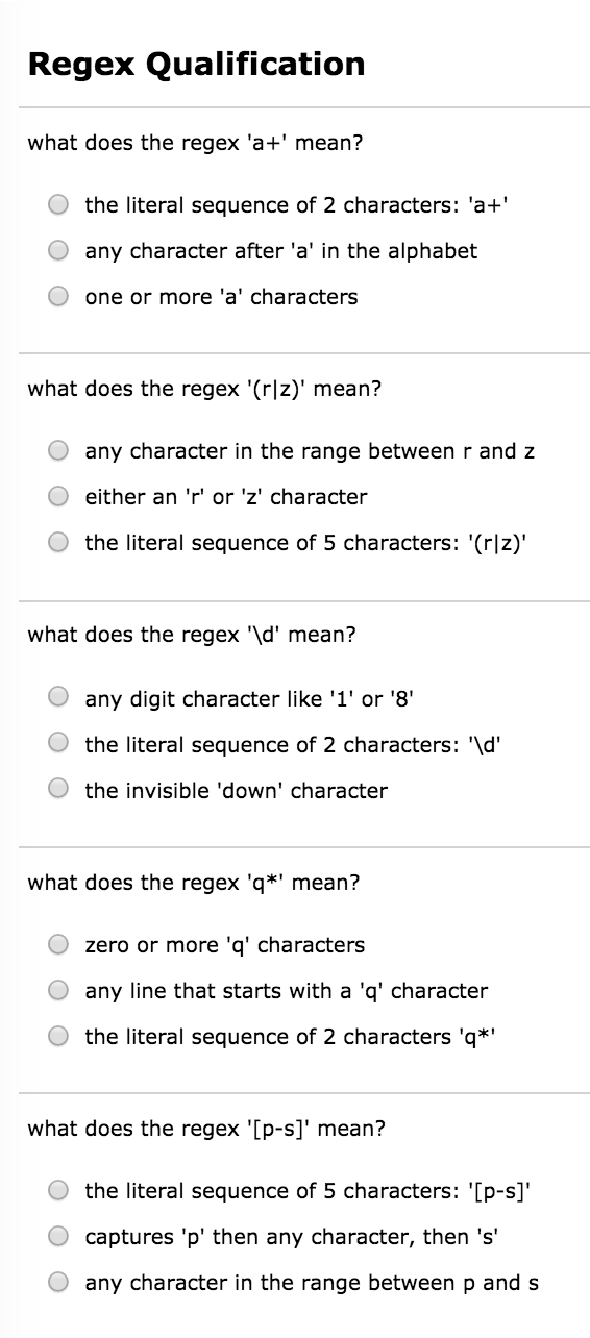
\includegraphics[height=20cm,keepaspectratio]{nontex/qualificationTest}
\vspace{-12pt}
\caption{The qualification test taken to participate in the regex understandability study.  Four out of five questions must be answered correctly.}
\vspace{-6pt}
\label{fig:qualTest}
\end{figure}

\section*{Template}
\label{app:MTtemplate}

\begin{figure}[ht]
   \centering
   \begin{tabular}{@{}c@{\hspace{.1cm}}c@{}}
       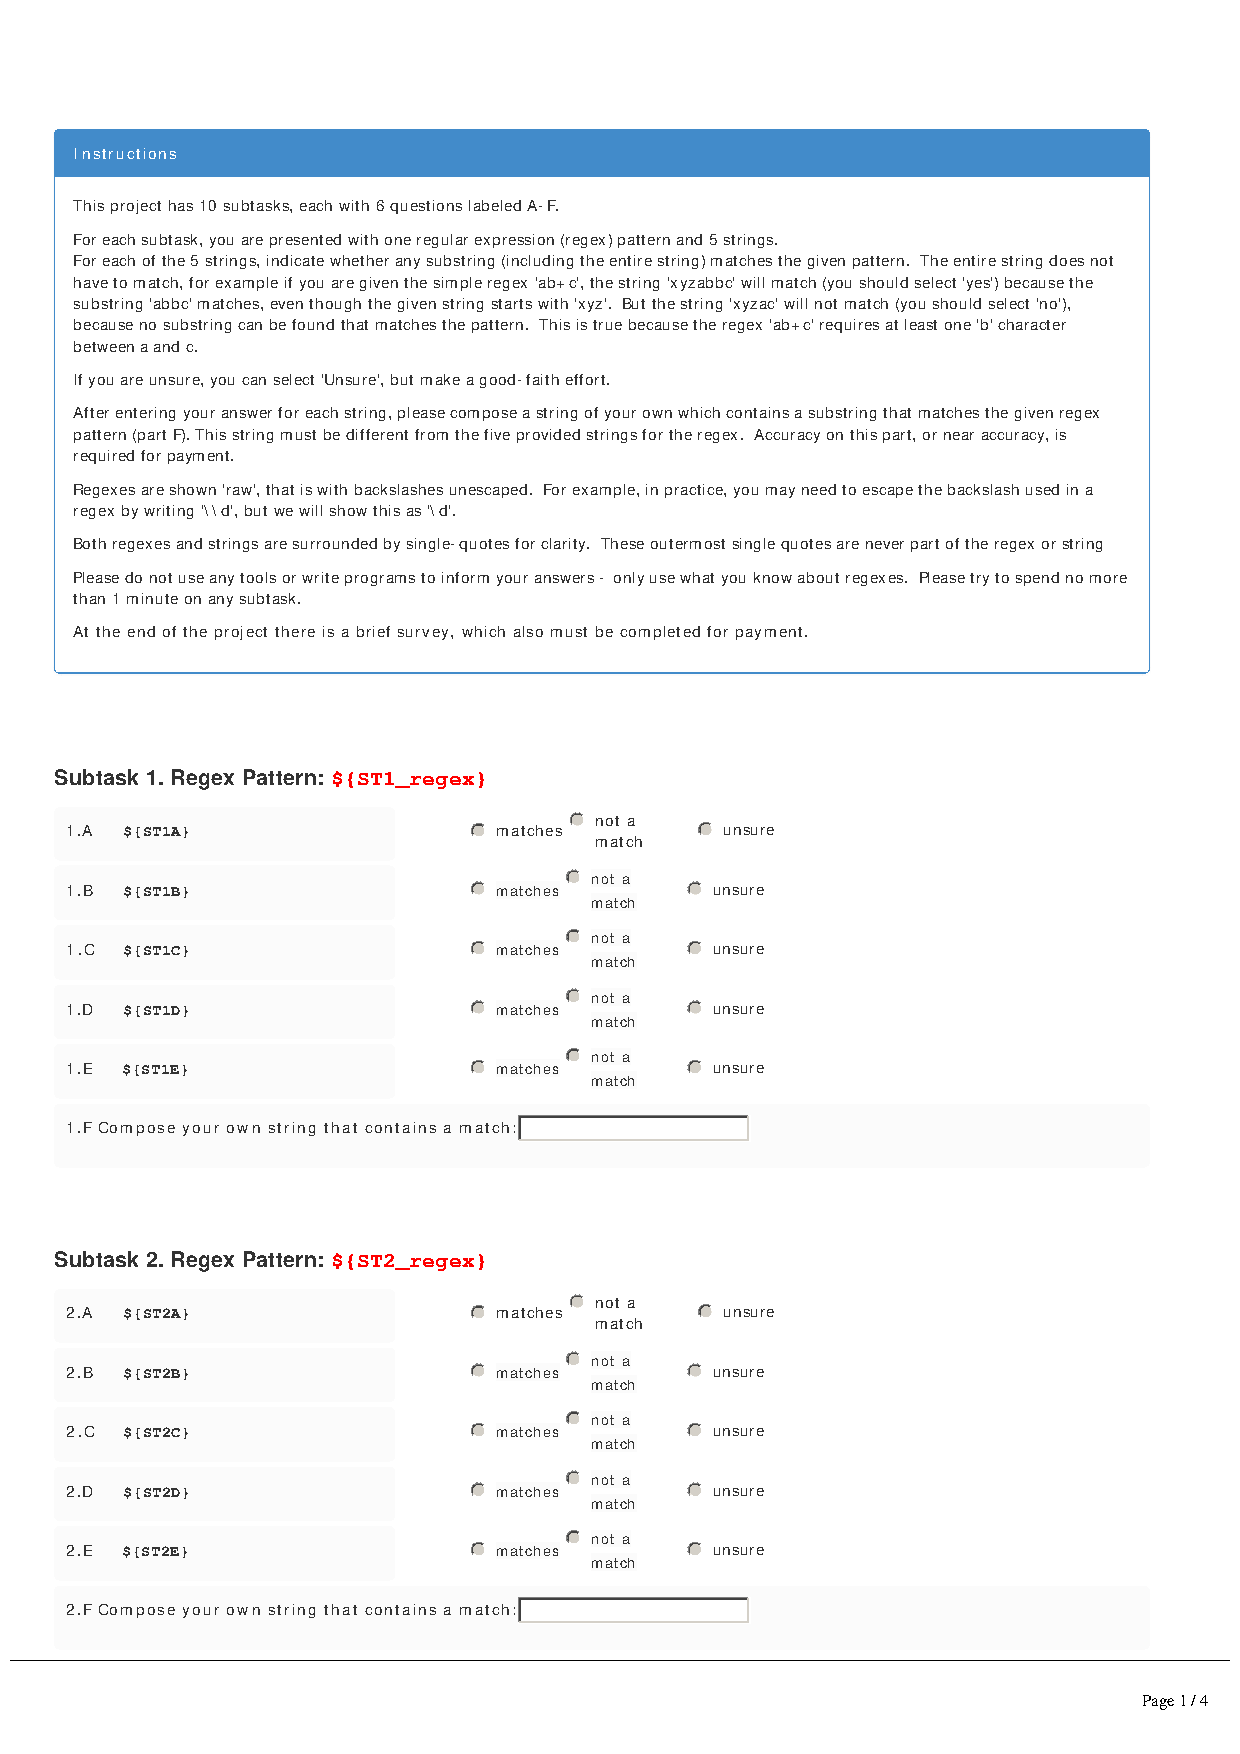
\includegraphics[page=1,width=.46\textwidth]{nontex/MTtemplate} &
       \includegraphics[page=2,width=.46\textwidth]{nontex/MTtemplate} \\[.1cm]
       \includegraphics[page=3,width=.46\textwidth]{nontex/MTtemplate} &
       \includegraphics[page=4,width=.46\textwidth]{nontex/MTtemplate} \\[.1cm]
   \end{tabular}
 \caption{Template for one HIT.  Red values like  \$\{ST1\_regex\} are populated with regexes, and black values like \$\{ST1A\} are populated with matching strings.}
 \label{fig:MTtemplate}
\end{figure}

\section*{Regexes And Matching Strings Tested On Mechanical Turk, Organized By Metagroup}
\label{app:MTstudyInput}

Metagroup 1: testing S1 vs S2
\vspace{-5mm}
\begin{multicols}{3}
\begin{itemize}[noitemsep,topsep=0pt]
\item[S1] \cverb!%([0-9A-Fa-f]{2})!
\item[S2] \begin{footnotesize}\cverb!%([0-9a-fA-F][0-9a-fA-F])!\end{footnotesize}
\item[] \verb|"g%a9"|
\item[] \verb|"%-F"|
\item[] \verb|"0123abC"|
\item[] \verb|"%0G"|
\item[] \verb|"%8F-1"|
\item[S1] \cverb!&d([aeiou]{2})z!
\item[S2] \cverb!&d([aeiou][aeiou])z!
\item[] \verb|"&deez"|
\item[] \verb|"t&dazz"|
\item[] \verb|"&diez"|
\item[] \verb|"&dazez"|
\item[] \verb|"douz"|
\item[S1] \cverb!fa[lmnop]{3}!
\item[S2] \cverb!fa[lmnop][lmnop][lmnop]!
\item[] \verb|"fall"|
\item[] \verb|"afmon"|
\item[] \verb|"fanopster"|
\item[] \verb|"infalobl"|
\item[] \verb|"famlnk"|
\end{itemize}
\end{multicols}
\vspace{-2mm}
Metagroup 2: testing C1 vs C4, focusing on DEC
\vspace{-5mm}
\begin{multicols}{3}
\begin{itemize}[noitemsep,topsep=0pt]
\item[C1] \cverb!([0-9]+)\.([0-9]+)!
\item[C4] \cverb!(\d+)\.(\d+)!
\item[] \verb|"11.3"|
\item[] \verb|"12."|
\item[] \verb|"888"|
\item[] \verb|"0a.2"|
\item[] \verb|".075"|
\item[C1] \cverb!xg1([0-9]{1,3})%!
\item[C4] \cverb!xg1(\d{1,3})%!
\item[] \verb|"1x1g1333%"|
\item[] \verb|"Lxg134%"|
\item[] \verb|"1492%"|
\item[] \verb|"xg13%"|
\item[] \verb|"xg1345%2"|
\item[C1] \cverb![a-f]([0-9]+)[a-f]!
\item[C4] \cverb![a-f](\d+)[a-f]!
\item[] \verb|"d912a"|
\item[] \verb|"h12f"|
\item[] \verb|"aff321"|
\item[] \verb|"123af"|
\item[] \verb|"aaa4a"|
\end{itemize}
\end{multicols}
\pagebreak
Metagroup 3: testing C1 vs C4, focusing on WRD
\vspace{-5mm}
\begin{multicols}{3}
\begin{itemize}[noitemsep,topsep=0pt]
\item[C1] \cverb!&([A-Za-z0-9_]+);!
\item[C4] \cverb![&(\w+);]!
\item[] \verb|"&&"|
\item[] \verb|"abc_;"|
\item[] \verb|"&&a_9;"|
\item[] \verb|"&aFF;"|
\item[] \verb|"&a-F;"|
\item[C1] \cverb!1q[A-Za-z0-9_][A-Za-z0-9_]!
\item[C4] \cverb![1q\w\w]!
\item[] \verb|"1q&&"|
\item[] \verb|"1aqabc_"|
\item[] \verb|"1qabc2"|
\item[] \verb|"a1q245"|
\item[] \verb|"1q\w\w"|
\item[C1] \cverb![tuv[A-Za-z0-9_]]!
\item[C4] \cverb![tuv\w]!
\item[] \verb|"tuv\w"|
\item[] \verb|"tuv&"|
\item[] \verb|"tuvx"|
\item[] \verb|"amtuv0"|
\item[] \verb|"pqtuv"|
\end{itemize}
\end{multicols}
\vspace{-2mm}
Metagroup 4: C4 vs (C3 or C2), covering the other defaults
\vspace{-5mm}
\begin{multicols}{3}
\begin{itemize}[noitemsep,topsep=0pt]
\item[C3] \cverb![^0-9A-Za-z]!
\item[C4] \cverb![\W_]!
\item[] \verb|"abc"|
\item[] \verb|"."|
\item[] \verb|"*1"|
\item[] \verb|"123"|
\item[] \verb|"}x"|
\item[C3] \cverb![^0-9]!
\item[C4] \cverb![\D]!
\item[] \verb|"84732211"|
\item[] \verb|"axb33"|
\item[] \verb|"*1"|
\item[] \verb|"123"|
\item[] \verb|"}x"|
\item[C2] \cverb![\t\r\f\n ]!
\item[C4] \cverb![\s]!
\item[] \verb|"ggg"|
\item[] \verb|"    l"|
\item[] \verb|"el ela"|
\item[] \verb|"tp11"|
\item[] \verb|"0123abC"|
\end{itemize}
\end{multicols}
\vspace{-2mm}
Metagroup 5: testing L2 vs L3 (note that the pair \cverb!\..*! and \cverb!\.+! on the left is not equivalent, due to an oversight - the first regex was meant to be \cverb!\.\.*!)
\vspace{-5mm}
\begin{multicols}{3}
\begin{itemize}[noitemsep,topsep=0pt]
\item[L2] \cverb!\..*!
\item[L3] \cverb!\.+!
\item[] \verb|"99"|
\item[] \verb|"..."|
\item[] \verb|"a dog."|
\item[] \verb|"."|
\item[] \verb|"abc"|
\item[L2] \cverb!zaa*!
\item[L3] \cverb!za+!
\item[] \verb|"qtmnzba"|
\item[] \verb|"qtzaaa"|
\item[] \verb|"za"|
\item[] \verb|"azazaza"|
\item[] \verb|"az"|
\item[L2] \cverb!RR*!
\item[L3] \cverb!R+!
\item[] \verb|"98"|
\item[] \verb|"R0R"|
\item[] \verb|"ARROW"|
\item[] \verb|"qRs"|
\item[] \verb|"qrs"|
\end{itemize}
\end{multicols}
\pagebreak

Metagroup 6: testing T1 vs T3
\vspace{-5mm}
\begin{multicols}{3}
\begin{itemize}[noitemsep,topsep=0pt]
\item[T1] \cverb!(\$\{)\d+(:[^}]+\})!
\item[T3] \cverb!([$][{])\d+(:[^}]+[}])!
\item[] \verb|"${881:}"|
\item[] \verb|"{12:-}"|
\item[] \verb|"${09.1::}"|
\item[] \verb|"${31:13}"|
\item[] \verb|"#${1:x22}"|
\item[T1] \cverb!t\.\$+\d+\*!
\item[T3] \cverb!t[.][$]+\d+[*]!
\item[] \verb|"t..5*"|
\item[] \verb|"ampty.*$0"|
\item[] \verb|"sit."|
\item[] \verb|"t.$111*"|
\item[] \verb|"qt.$$$41*"|
\item[T1] \cverb!\{\$(\d+\.\d)\}!
\item[T3] \cverb![{][$](\d+[.]\d)[}]!
\item[] \verb|"{$88.\}"|
\item[] \verb|"{$0.3}"|
\item[] \verb|"$99.2"|
\item[] \verb|"{$31.13}"|
\item[] \verb|"{$112.4}"|
\end{itemize}
\end{multicols}
Metagroup 7: testing D1 vs D2 vs D3
\vspace{-5mm}
\begin{multicols}{2}
\begin{itemize}[noitemsep,topsep=0pt]
\item[D1] \cverb!((q4f){0,1}ab)!
\item[D2] \cverb!((q4f)?ab)!
\item[D3] \cverb!(q4fab|ab)!
\item[] \verb|"ab"|
\item[] \verb|"fq4f"|
\item[] \verb|"xyzq4fab"|
\item[] \verb|"zlmab"|
\item[] \verb|"qfa4"|
\item[D1] \cverb!(dee(do){1,2})!
\item[D2] \cverb!(deedo(do)?)!
\item[D3] \cverb!(deedo|deedodo)!
\item[] \verb|"do deedodeedo"|
\item[] \verb|"dodeedee do"|
\item[] \verb|"do deedodo"|
\item[] \verb|"dedoode"|
\item[] \verb|"deedo do"|
\end{itemize}
\end{multicols}
\vspace{-2mm}
Metagroup 8: testing C1 vs C2 vs C5
\vspace{-5mm}
\begin{multicols}{2}
\begin{itemize}[noitemsep,topsep=0pt]
\item[C1] \cverb!tri[a-f]3!
\item[C2] \cverb!tri[abcdef]3!
\item[C5] \cverb!tri(a|b|c|d|e|f)3!
\item[] \verb|"tri3def"|
\item[] \verb|"triabc3"|
\item[] \verb|"tric3"|
\item[] \verb|"trig3"|
\item[] \verb|"abc3"|
\item[C1] \cverb!no[w-z]5!
\item[C2] \cverb!no[wxyz]5!
\item[C5] \cverb!no(w|x|y|z)5!
\item[] \verb|"nov5"|
\item[] \verb|"noxy5"|
\item[] \verb|"now5"|
\item[] \verb|"ny5"|
\item[] \verb|"noz"|
\end{itemize}
\end{multicols}
\pagebreak

Metagroup 9: testing C2/T1 vs C5/T1 vs C2/T4 (provides T1 vs T4 and C2 vs C5)
\vspace{-5mm}
\begin{multicols}{2}
\begin{itemize}[noitemsep,topsep=0pt]
\item[C2/T1] \cverb!([}{])!
\item[C5/T1] \cverb!(\{|\})!
\item[C2/T4] \cverb!([\072\073])!
\item[] \verb|"{o0ps"|
\item[] \verb|"|"|
\item[] \verb|"{x}"|
\item[] \verb|"([c])"|
\item[] \verb|"pcm}"|
\item[C2/T1] \cverb!([:;])!
\item[C5/T1] \cverb!(:|;)!
\item[C2/T4] \cverb!([\0175\0173])!
\item[] \verb|";o0ps"|
\item[] \verb|"|"|
\item[] \verb|":x"|
\item[] \verb|"([c])"|
\item[] \verb|"pcm;:"|
\end{itemize}
\end{multicols}
\vspace{-2mm}
Metagroup 10: testing C1/T2 vs C1/T4 vs C2/T1 (provides only T2 vs T4)
\vspace{-5mm}
\begin{multicols}{2}
\begin{itemize}[noitemsep,topsep=0pt]
\item[C1/T2] \cverb!xyz[\x5b-\x5f]!
\item[C1/T4] \cverb!xyz[\0133-\0140]!
\item[C2/T1] \cverb!xyz[_\[\]`\^\\]!
\item[] \verb|"xyz_1"|
\item[] \verb|"yzx'3"|
\item[] \verb|"xyzyx"|
\item[] \verb|"xyz\133"|
\item[] \verb|"xyz139"|
\item[C1/T2] \cverb!t[\x3a-\x3b]+p!
\item[C1/T4] \cverb!t[\072-\073]+p!
\item[C2/T1] \cverb!t[:;]+p!
\item[] \verb|"t;;p"|
\item[] \verb|"t}p"|
\item[] \verb|"t\73p"|
\item[] \verb|"t:;:p"|
\item[] \verb|"t::;:"|
\end{itemize}
\end{multicols}
